\section{A More Detailed Explanation of Goodhart's Law}\label{appendix:extra_explanation}

In this section, we provide an intuitive explanation of why Goodharting occurs in MDPs, that will be more detailed an clear than the explanation provided in Section~\ref{sec:explain_goodhart}.

First of all, as in Section~\ref{sec:explain_goodhart}, recall that $\J_\R(\policy) = \occmeas{\policy} \cdot \R$, where $\occmeas{\policy}$ is the occupancy measure of $\pi$. This means that we can decompose $\J_\R$ into two steps, the first of which is independent of $R$, and maps $\Policies$ to $\Polytope$, and the second of which is a linear function.
Recall also that $\Polytope$ is a convex polytope.
Therefore, the problem of finding an optimal policy can be viewed as maximising a linear function within a convex polytope $\Polytope$. If $R_1$ is the reward function we are optimising, then we can visualise this as follows:

\begin{figure}[h]
    \centering
    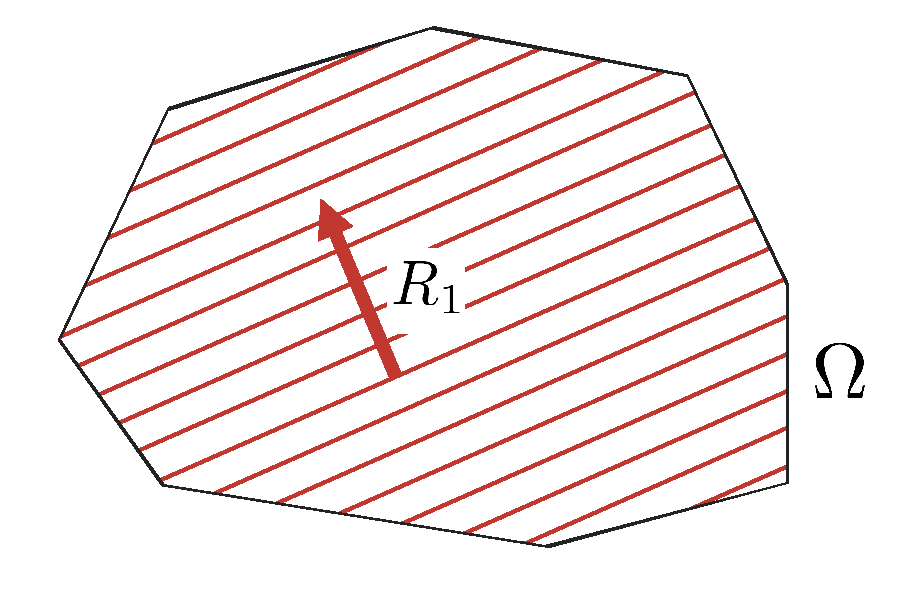
\includegraphics[width=0.5\linewidth]{other_figures/explanatory_pictures/exp1.pdf}
    %\caption{text.}
    %\label{diagram:goodharting1}
\end{figure}

Here the red arrow denotes the direction of $R_1$ within $\Polytope$. Note that this direction corresponds to $\QProj_\T \R_1$, rather than $R_1$, since $\Polytope$ lies in a lower-dimensional affine subspace. Similarly, the red lines correspond to the level sets of $R_1$, i.e.\ the directions we can move in without changing $R_1$.

Now, if $R_1$ is a \emph{proxy reward}, then we may assume that there is also some (unknown) true reward function $R_0$. This reward also induces a linear function on $\Polytope$:

\begin{figure}[h]
    \centering
    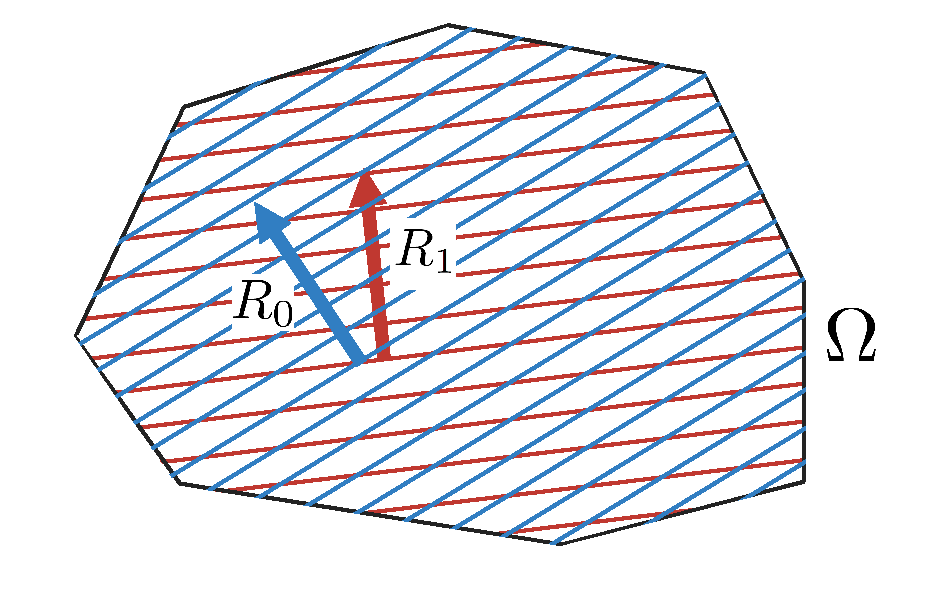
\includegraphics[width=0.5\linewidth]{other_figures/explanatory_pictures/exp2.pdf}
    %\caption{text.}
    %\label{diagram:goodharting1}
\end{figure}

Suppose we pick a random point $\occmeas{\policy}$ in $\Polytope$, and then move in a direction that increases $\occmeas{\policy} \cdot R_1$. This corresponds to picking a random policy $\pi$, and then modifying it in a direction that increases $\J_{\ProxR}(\policy)$.
In particular, let us consider what happens to the true reward function $R_0$, as we move in the direction that most rapidly increases the proxy reward $R_1$.

To start with, if we are in the interior of $\Polytope$ (i.e., not close to any constraints), then the direction that most rapidly increases $R_1$ is to move parallel to $\QProj_\T \R_1$. Moreover, if the angle $\theta$ between $\QProj_\T \R_1$ and $\QProj_\T \R_0$ is no more than $\pi/2$, then this is guaranteed to also increase the value of $R_0$. To see this, simply consider the following diagram:

\begin{figure}[H]
    \centering
    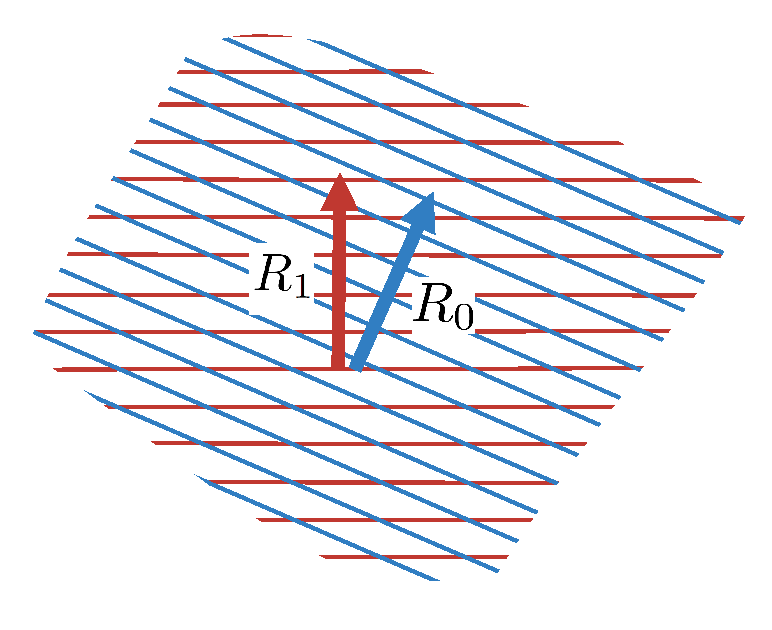
\includegraphics[width=0.5\linewidth]{other_figures/explanatory_pictures/exp3.pdf}
    %\caption{text.}
    %\label{diagram:goodharting1}
\end{figure}

However, as we move parallel to $\QProj_\T \R_1$, we will eventually hit the boundary of $\Polytope$. When we do this, the direction that most rapidly increases $R_1$ will no longer be parallel to $\QProj_\T \R_1$. Instead, it will be parallel to the projection of $R_1$ onto the boundary of $\Polytope$ that we just hit. Moreover, if we keep moving in \emph{this} direction, then we might no longer be increasing the true reward $R_0$. To see this, consider the following diagram:

\begin{figure}[h]
    \centering
    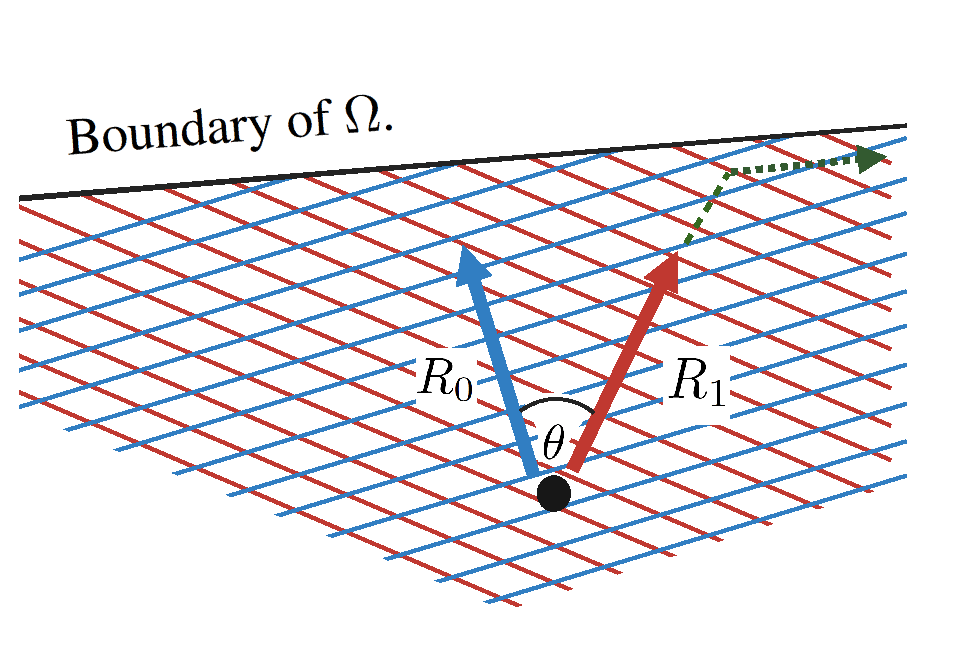
\includegraphics[width=0.5\linewidth]{other_figures/explanatory_pictures/exp4.pdf}
    %\caption{text.}
    %\label{diagram:goodharting1}
\end{figure}

The dashed green line corresponds to the path that most rapidly increases $R_1$. As we move along this path, $R_0$ initially increases. However, after the path hits the boundary of $\Polytope$ and changes direction, $R_0$ will instead start to decrease. Thus, if we were to plot $\J_{R_1}(\pi)$ and $\J_{R_0}(\pi)$ over time, we would get a plot that looks roughly like this:

\begin{figure}[H]
    \centering
    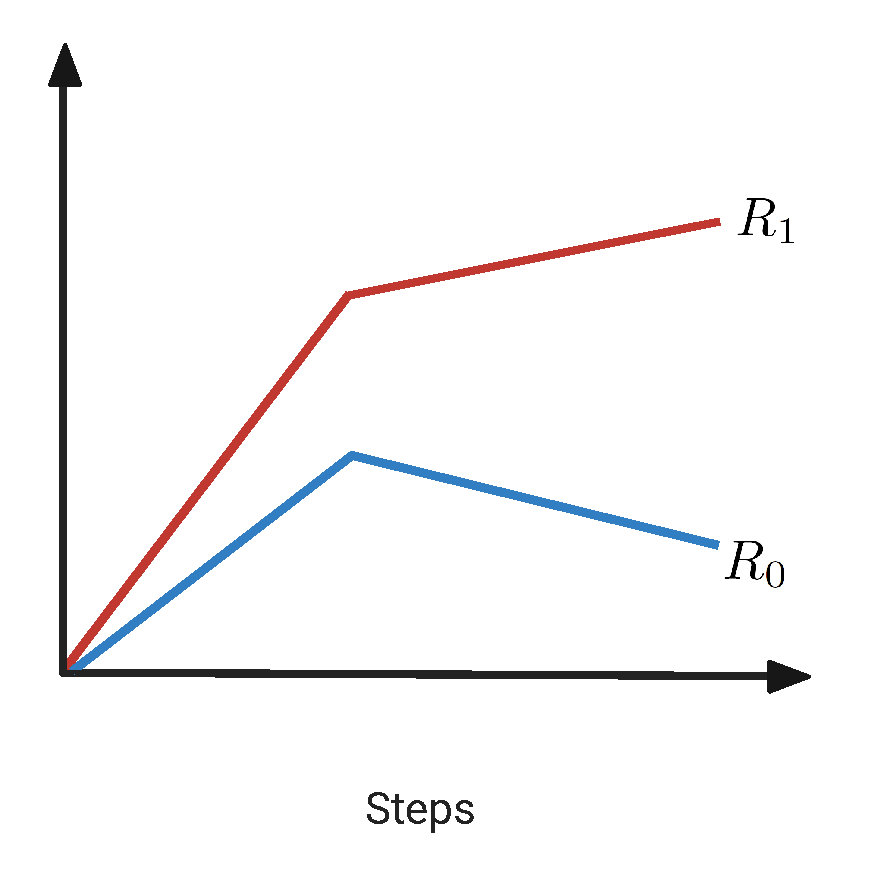
\includegraphics[width=0.4\linewidth]{other_figures/explanatory_pictures/graph1.pdf}
    %\caption{text.}
    \label{fig:goodharting-linear-decrease}
\end{figure}

Next, it is important to note that $R_0$ is not guaranteed to decrease after we hit the boundary of $\Polytope$. To see this, consider the following diagram:

\begin{figure}[ht]
    \centering
    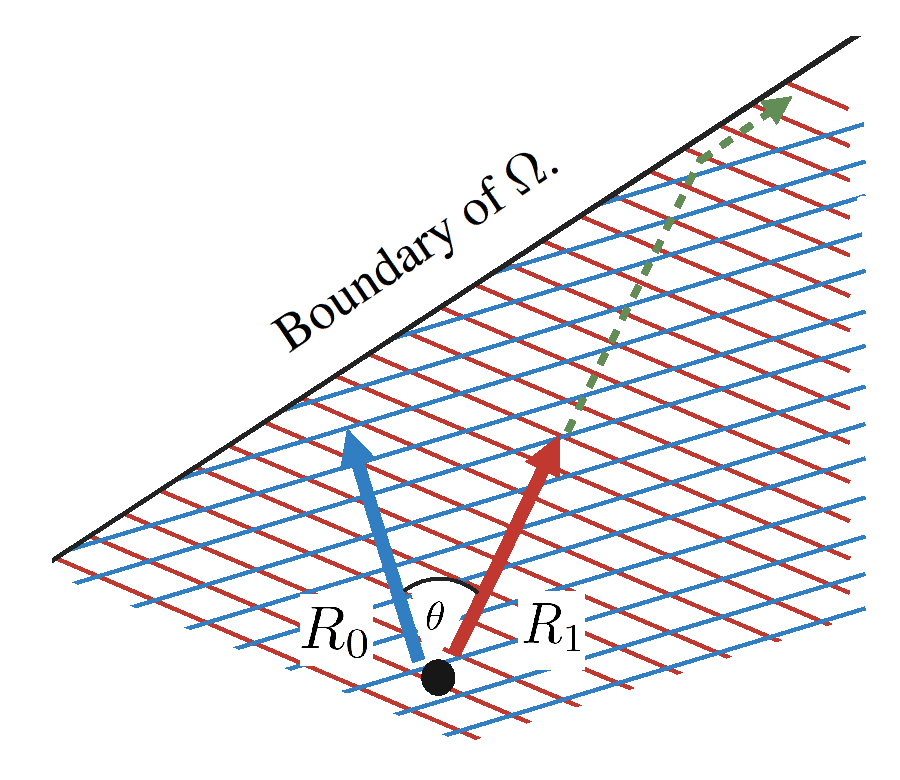
\includegraphics[width=0.5\linewidth]{other_figures/explanatory_pictures/exp5.pdf}
    %\caption{text.}
    %\label{diagram:goodharting1}
\end{figure}

The dashed green line again corresponds to the path that most rapidly increases $R_1$. As we move along this path, $R_0$ will increase both before and after the path has hit the boundary of $\Polytope$. If we were to plot $\J_{R_1}(\pi)$ and $\J_{R_0}(\pi)$ over time, we would get a plot that looks roughly like this:

\begin{figure}[h]
    \centering
    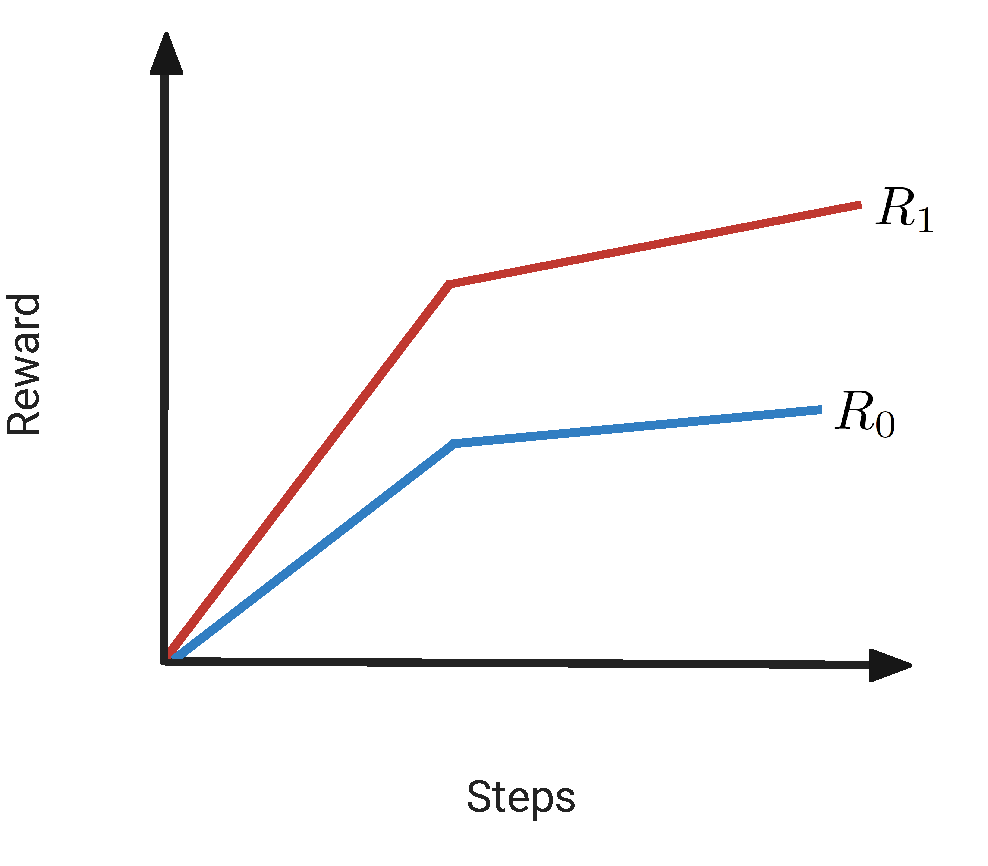
\includegraphics[width=0.5\linewidth]{other_figures/explanatory_pictures/graph2.pdf}
    \label{fig:goodharting-linear-increase}
    % \caption{}
\end{figure}

The next thing to note is that we will not just hit the boundary of $\Polytope$ once. If we pick a random point $\occmeas{\policy}$ in $\Polytope$, and keep moving in the direction that most rapidly increases $\occmeas{\policy} \cdot R_1$ until we have found the maximal value of $R_1$ in $\Polytope$, then we will hit the boundary of $\Polytope$ over and over again. Each time we hit this boundary we will change the direction that we are moving in, and each time this happens, there is a risk that we will start moving in a direction that decreases $R_0$.

Note that Goodharting corresponds to the case where we follow a path through $\Polytope$ along which $R_0$ initially increases, but eventually starts to decrease. As we have seen, this must be caused by the boundaries of $\Polytope$.
We may now ask; under what conditions do these boundaries force the path of steepest ascent (of $R_1$) to move in a direction that decreases $R_0$? By inspecting the above diagrams, we can see that this depends on the angle between the normal vector of that boundary and $\QProj_\T R_1$, and the angle between $\QProj_\T R_1$ and $\QProj_\T R_0$. In particular, in order for $R_0$ to start decreasing, it has to be the case that the angle between $\QProj_\T R_1$ and $\QProj_\T R_0$ is \emph{larger} than the angle between $\QProj_\T R_1$ and the normal vector of the boundary of $\Polytope$. This immediately tells us that if the angle between $\QProj_\T R_1$ and $\QProj_\T R_0$ is small (i.e., if $\mathrm{arg}(R_0, R_1)$ is small), then Goodharting will be less likely to occur. 

Moreover, as the angle between $\QProj_\T R_1$ and the normal vector of the boundary of $\Polytope$ becomes \emph{smaller}, Goodharting should be correspondingly \emph{more} likely to occur. Next, recall that Proposition~\ref{prop:concave_proof} tells us that this angle will decrease monotonically along the path of steepest ascent (of $R_1$). As such, Goodharting will get more and more likely, the further we move along the path of steepest ascent. This explains why Goodharting becomes more likely when more optimisation pressure is applied. 
